% This is a sample input file for the 
% Journal of Language Modelling
%
% Please consult jlm-guidelines.pdf as well.
%
% The file has to be encoded in UTF-8.

% Obligatory document class:
\documentclass[
% remove this option after the review phase:
    anonymous,
% activate this option if traditional TeX notation for dashes (--) and
% double quotes (`` '') is required:
%    TeXligs
]{jlm}

% Standard LaTeX tool for including external graphics
% (needed only if your text contains illustrations):
\usepackage{graphicx}



% AUTHOR-PROVIDED LaTeX COMMANDS %%%%%%%%%%%%%%%%%%%%%%%%%%%%
%
% Please place your own definitions and macros below.  Do not put
% any macro-definitions within the text body.

%%%%%%%%%%%%%%%%%%%%%%%%%%%%%%%%%%%%%%%%%%%%%%%%%%%%%%%%%%%%%

\begin{document}

\title{A Method for Retroisotonal Blabalysis\\ of a Parallel
  Stream of Volatile Aromas\\
  in the Semi-quasi-space}

% If the title is too long for the running head, please provide a
% shorter version here:
% (Otherwise leave this command commented out.)
\titlerunning{Retroisotonal Blabalysis of Volatile Aromas}


% If all authors have the same affiliation do not use the \inst
% command: 
\author{Filigran Fifak\inst{1}
  \and Gizbert Gryzogrzechotalski\inst{2}
  \and Jeffrey Johansen\inst{2}
  \and David Drake\inst{1}
  \and Craig Cadr\inst{3}
  \and Kim~K.~Kominsky\inst{4}
  \and Zachary Zweistein\inst{1,3}
}

% If there are more than two authors, please abbreviate author list
% for running heads:
\authorrunning{Filigran Fifak et al.}

% Affiliations of authors separated with \and:
\affiliation{%
  Institute of Blabal Fetoria, Fid\^o F\'o\`oish University of Fafia,
  Fafia, Fifa
  \and 
  Institute of Computer Science, Polish Academy of Sciences, Warsaw,
  Poland
  \and
  Princeton University, Princeton, USA
  \and 
  Warsaw University of Technology, Warsaw, Poland 
}

\keywords{blabalysis, volatile~aromas}


\maketitle              % typesets the title

\begin{abstract}
  The abstract should summarise the contents of the paper in at least
  70 and at most 150 words.  The present paper has no scientific
  relevance and should be used as a practical example of text
  formatting for the Journal of Language Modelling.
\end{abstract}

\section{Unicode input files\\ in the 21 century}

This is an example article for JLM.  You can use arbitrary Unicode
characters in your file, provided they are present in the font:
αβγδρπ, «Какво е това?», naïve, crème brûlée, ˌpʃɛpjurˈkɔfskʲi,
‣≤≥⅓⅔.

Please note, that the traditional \TeX\ notation for dashes and double
quotes has to be
activated with the \texttt{TeXligs} option, if desired:\\
e--f g–h ``a'' “b” `c' ‘d’\\
\texttt{e--f g–h ``a'' “b” `c' ‘d’}\\
\textsf{e--f g–h ``a'' “b” `c' ‘d’}.



\section{Important remarks\\ on the usage of references}

We strongly suggest using author-year references, which are easier to
follow for the reader than numerical identifiers
\citep[cf.][]{fifak:sigma_rho}.  The class internally loads the
\texttt{natbib} package for that purpose.  Please employ the
\verb+\citet+ command when referring to the author(s), as advised by
\citet{fifak:sigma_rho} or works cited, and \verb+\citep+ – only for
parenthetical references \citep{fifak:sigma_rho}.


The bibliography should be ordered alphabetically \citep[pp.
20–22]{blarbarucki:blabalyser}, which can be achieved automatically
using Bib\TeX\ and the bibliographical style \texttt{jlm} used in this
example \citep{blarbarucki:blabalyser,fifak:aspects,fifak:blabal}.



\section{Illustrations and tables}


\subsection{Illustrations}
\label{sec:illustrations}

Your figures \emph{must} be available in formats accepted by \XeLaTeX{}
(PDF, PNG, JPEG, PGF/TikZ). To include them in your document it is
advisable to use the standard package \texttt{graphicx} (see the
example in Figure~\ref{fig:ex}).
\begin{figure}
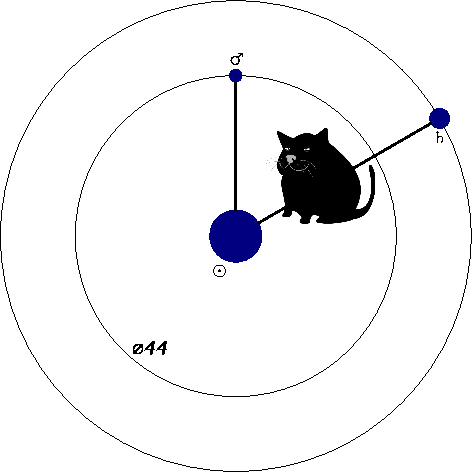
\includegraphics{jlm-example-fig1-k44}
\caption{An example of an included figure}
\label{fig:ex}
\end{figure}


When preparing figures with external programs, please consider the
following suggestions:
\begin{itemize}
\item The printed version of the journal will be in black and white.
  Please check that your figure is readable when stripped out of
  colour.  The pictures can, however, be in colour for the benefit of
  the on-line version.
\item Prefer vector graphics formats, which will not deteriorate when
  scaled.
\item If a bitmap is unavoidable, use a resolution of at least 300~dpi
  (with the obvious exception of screen shots).
\item Do not use lossy JPEG compression for screen shots nor line
  graphics (in particular for pictures containing textual elements).
\end{itemize}

\subsection{Tables}
\label{sec:tables}


Over-wide tables have to be reduced to the page width.  You can reduce
the inter-column distances in such tables (the \verb|\tabcolsep|
parameter), rotate the table and place it as a full-page float, or use
a \verb|\small| font (if there is no other possibility).

\begin{table}

\caption{Values of some aspects}

\renewcommand{\arraystretch}{1.4}
\begin{tabular}{r|rrrrrl}
\hline
house &
\multicolumn1c{ʘ} & α\textsubscript{Cent} & \emph{M₃₁} & $\approx$
  & \rlap{−}×
  & \multicolumn1{c}{ᴥ} \\
\hline
 1 & 0.43 & 102 & 12.4 & 4 & 2 & 1asp \\
 3 & 0.45 & 412 & 32.6 & 14 & 7 & 4kid \\
 7 & 0.16 & 111 & 92.1 & 3 & 9 & 2mer\\
12 & 0.49 & 224 & 25.5 & 1 & 1 & 4asp\\
\hline
\end{tabular}
\label{tab:ex}
\end{table}

Elements like Section \ref{sec:illustrations}, Figure~\ref{fig:ex},
Table~\ref{tab:ex}, and Equation~(\ref{eq:ex}) can be referenced
symbolically if you provide respective labels (see the source code for
this document).

For math you can use all constructs provided by the \texttt{amsmath}
package, e.g.:
\begin{align}
a & =  c + d  , \\
e & =  f - d  , \label{eq:ex}\\
g & =  \sum_{\substack{
0\le i\le m\\
0<j<n}}
P_\infty(i,j)\times\mathbf{\Delta} , \notag\\
h &= (\alpha-\beta)\cdot\biggl[\sum_i a_i\Bigl\lvert\sum_j
x_{ij}\Bigr\rvert^p\biggr]^{1/p} .
\end{align}


\section{The reviewing process}

The journal uses a double-blind reviewing process.  Your article
should be made anonymous before sending to the reviewers.  When
submitting your paper please use the \texttt{[anonymous]} option of
the document class (see the header of this example), which will remove
the names and affiliations of the authors from the title page.  Please
note, however, that you may have other identifying elements in your text
(especially in references), which you should adapt accordingly.

When the article is accepted these changes should be reverted.  The
final version should contain a complete list of authors and their
affiliations.


\bibliographystyle{jlm}
\bibliography{example-bibdata}


\end{document}


%%% Local Variables:
%%% mode: latex
%%% mode: flyspell
%%% TeX-master: t
%%% TeX-engine: xetex
%%% TeX-PDF-mode: t
%%% coding: utf-8
%%% ispell-local-dictionary: "british"
%%% End:
